{
\begin{figure}
    \begin{subfigure}[t]{0.2\textwidth}
        \centering
        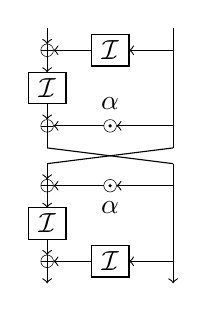
\begin{tikzpicture}[xscale=0.8, yscale=-0.4]
            \draw [->] (0,0) -- (0,0.5);
            \draw [very thin] (0,0.7) ellipse (0.1 and 0.2);
            \draw [very thin] (0,0.5) -- (0,0.9);
            \draw [very thin] (-0.1,0.7) -- (0.1,0.7);
            \draw (2,0) -- (2,0.7);
            \draw [->] (2,0.7) -- (1.3,0.7);
            \draw (0.7,0.2) rectangle (1.3,1.2) node[pos=0.5] {$\mathcal{I}$};
            \draw [->] (0.7,0.7) -- (0.1,0.7);
            \draw [->] (0,0.9) -- (0,1.4);
            \draw (-0.3,1.4) rectangle (0.3,2.4) node[pos=0.5] {$\mathcal{I}$};
            \draw [->] (0,2.4) -- (0,2.9);
            \draw [very thin] (0,3.1) ellipse (0.1 and 0.2);
            \draw [very thin] (0,2.9) -- (0,3.3);
            \draw [very thin] (-0.1,3.1) -- (0.1,3.1);
            \draw (2,0.7) -- (2,3.1);
            \draw [->] (2,3.1) -- (1.1,3.1);
            \draw [very thin] (1,3.1) ellipse (0.1 and 0.2);
            \fill[black] (1,3.1) ellipse (0.0285714285714 and 0.0571428571429);
            \draw (1,2.9) node[anchor=south] {$\alpha$};
            \draw [->] (0.9,3.1) -- (0.1,3.1);
            \draw (0,3.3) -- (0,3.8);
            \draw (2,3.1) -- (2,3.8);
            \draw (2,3.8) -- (0,4.3);
            \draw (0,3.8) -- (2,4.3);
            \draw [->] (0,4.3) -- (0,4.8);
            \draw [very thin] (0,5) ellipse (0.1 and 0.2);
            \draw [very thin] (0,4.8) -- (0,5.2);
            \draw [very thin] (-0.1,5) -- (0.1,5);
            \draw (2,4.3) -- (2,5);
            \draw [->] (2,5) -- (1.1,5);
            \draw [very thin] (1,5) ellipse (0.1 and 0.2);
            \fill[black] (1,5) ellipse (0.0285714285714 and 0.0571428571429);
            \draw (1,5.2) node[anchor=north] {$\alpha$};
            \draw [->] (0.9,5) -- (0.1,5);
            \draw [->] (0,5.2) -- (0,5.7);
            \draw (-0.3,5.7) rectangle (0.3,6.7) node[pos=0.5] {$\mathcal{I}$};
            \draw [->] (0,6.7) -- (0,7.2);
            \draw [very thin] (0,7.4) ellipse (0.1 and 0.2);
            \draw [very thin] (0,7.2) -- (0,7.6);
            \draw [very thin] (-0.1,7.4) -- (0.1,7.4);
            \draw (2,5) -- (2,7.4);
            \draw [->] (2,7.4) -- (1.3,7.4);
            \draw (0.7,6.9) rectangle (1.3,7.9) node[pos=0.5] {$\mathcal{I}$};
            \draw [->] (0.7,7.4) -- (0.1,7.4);
            \draw [->] (0,7.6) -- (0,8.1);
            \draw [->] (2,7.4) -- (2,8.1);
        \end{tikzpicture}
        \FigDef{affine-classes-none}{No swaps}
    \end{subfigure}
    \hspace{0.2cm}
    \begin{subfigure}[t]{0.2\textwidth}
        \centering
        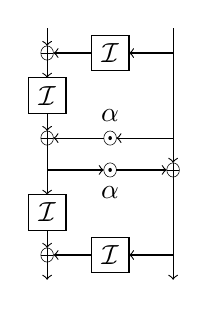
\begin{tikzpicture}[xscale=0.8, yscale=-0.45]
            \draw [->] (0,0) -- (0,0.5);
            \draw [very thin] (0,0.7) ellipse (0.1 and 0.2);
            \draw [very thin] (0,0.5) -- (0,0.9);
            \draw [very thin] (-0.1,0.7) -- (0.1,0.7);
            \draw (2,0) -- (2,0.7);
            \draw [->] (2,0.7) -- (1.3,0.7);
            \draw (0.7,0.2) rectangle (1.3,1.2) node[pos=0.5] {$\mathcal{I}$};
            \draw [->] (0.7,0.7) -- (0.1,0.7);
            \draw [->] (0,0.9) -- (0,1.4);
            \draw (-0.3,1.4) rectangle (0.3,2.4) node[pos=0.5] {$\mathcal{I}$};
            \draw [->] (0,2.4) -- (0,2.9);
            \draw [very thin] (0,3.1) ellipse (0.1 and 0.2);
            \draw [very thin] (0,2.9) -- (0,3.3);
            \draw [very thin] (-0.1,3.1) -- (0.1,3.1);
            \draw (2,0.7) -- (2,3.1);
            \draw [->] (2,3.1) -- (1.1,3.1);
            \draw [very thin] (1,3.1) ellipse (0.1 and 0.2);
            \fill[black] (1,3.1) ellipse (0.0285714285714 and 0.0571428571429);
            \draw (1,2.9) node[anchor=south] {$\alpha$};
            \draw [->] (0.9,3.1) -- (0.1,3.1);
            \draw (0,3.3) -- (0,4);
            \draw [->] (2,3.1) -- (2,3.8);
            \draw [very thin] (2,4) ellipse (0.1 and 0.2);
            \draw [very thin] (2,3.8) -- (2,4.2);
            \draw [very thin] (1.9,4) -- (2.1,4);
            \draw [->] (0,4) -- (0.9,4);
            \draw [very thin] (1,4) ellipse (0.1 and 0.2);
            \fill[black] (1,4) ellipse (0.0285714285714 and 0.0571428571429);
            \draw (1,4.2) node[anchor=north] {$\alpha$};
            \draw [->] (1.1,4) -- (1.9,4);
            \draw [->] (0,4) -- (0,4.7);
            \draw (-0.3,4.7) rectangle (0.3,5.7) node[pos=0.5] {$\mathcal{I}$};
            \draw [->] (0,5.7) -- (0,6.2);
            \draw [very thin] (0,6.4) ellipse (0.1 and 0.2);
            \draw [very thin] (0,6.2) -- (0,6.6);
            \draw [very thin] (-0.1,6.4) -- (0.1,6.4);
            \draw (2,4.2) -- (2,6.4);
            \draw [->] (2,6.4) -- (1.3,6.4);
            \draw (0.7,5.9) rectangle (1.3,6.9) node[pos=0.5] {$\mathcal{I}$};
            \draw [->] (0.7,6.4) -- (0.1,6.4);
            \draw [->] (0,6.6) -- (0,7.1);
            \draw [->] (2,6.4) -- (2,7.1);
        \end{tikzpicture}
        \FigDef{affine-classes-after}{Swap after}
    \end{subfigure}
    \hspace{0.2cm}
    \begin{subfigure}[t]{0.2\textwidth}
        \centering
        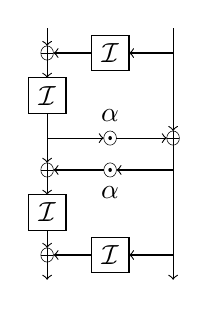
\begin{tikzpicture}[xscale=0.8, yscale=-0.45]
            \draw [->] (0,0) -- (0,0.5);
            \draw [very thin] (0,0.7) ellipse (0.1 and 0.2);
            \draw [very thin] (0,0.5) -- (0,0.9);
            \draw [very thin] (-0.1,0.7) -- (0.1,0.7);
            \draw (2,0) -- (2,0.7);
            \draw [->] (2,0.7) -- (1.3,0.7);
            \draw (0.7,0.2) rectangle (1.3,1.2) node[pos=0.5] {$\mathcal{I}$};
            \draw [->] (0.7,0.7) -- (0.1,0.7);
            \draw [->] (0,0.9) -- (0,1.4);
            \draw (-0.3,1.4) rectangle (0.3,2.4) node[pos=0.5] {$\mathcal{I}$};
            \draw (0,2.4) -- (0,3.1);
            \draw [->] (2,0.7) -- (2,2.9);
            \draw [very thin] (2,3.1) ellipse (0.1 and 0.2);
            \draw [very thin] (2,2.9) -- (2,3.3);
            \draw [very thin] (1.9,3.1) -- (2.1,3.1);
            \draw [->] (0,3.1) -- (0.9,3.1);
            \draw [very thin] (1,3.1) ellipse (0.1 and 0.2);
            \fill[black] (1,3.1) ellipse (0.0285714285714 and 0.0571428571429);
            \draw (1,2.9) node[anchor=south] {$\alpha$};
            \draw [->] (1.1,3.1) -- (1.9,3.1);
            \draw [->] (0,3.1) -- (0,3.8);
            \draw [very thin] (0,4) ellipse (0.1 and 0.2);
            \draw [very thin] (0,3.8) -- (0,4.2);
            \draw [very thin] (-0.1,4) -- (0.1,4);
            \draw (2,3.3) -- (2,4);
            \draw [->] (2,4) -- (1.1,4);
            \draw [very thin] (1,4) ellipse (0.1 and 0.2);
            \fill[black] (1,4) ellipse (0.0285714285714 and 0.0571428571429);
            \draw (1,4.2) node[anchor=north] {$\alpha$};
            \draw [->] (0.9,4) -- (0.1,4);
            \draw [->] (0,4.2) -- (0,4.7);
            \draw (-0.3,4.7) rectangle (0.3,5.7) node[pos=0.5] {$\mathcal{I}$};
            \draw [->] (0,5.7) -- (0,6.2);
            \draw [very thin] (0,6.4) ellipse (0.1 and 0.2);
            \draw [very thin] (0,6.2) -- (0,6.6);
            \draw [very thin] (-0.1,6.4) -- (0.1,6.4);
            \draw (2,4) -- (2,6.4);
            \draw [->] (2,6.4) -- (1.3,6.4);
            \draw (0.7,5.9) rectangle (1.3,6.9) node[pos=0.5] {$\mathcal{I}$};
            \draw [->] (0.7,6.4) -- (0.1,6.4);
            \draw [->] (0,6.6) -- (0,7.1);
            \draw [->] (2,6.4) -- (2,7.1);
        \end{tikzpicture}
        \FigDef{affine-classes-before}{Swap before}
    \end{subfigure}
    \hspace{0.2cm}
    \begin{subfigure}[t]{0.25\textwidth}
        \centering
        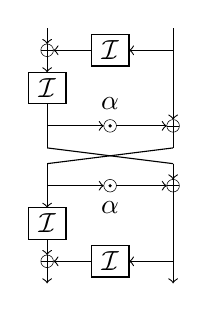
\begin{tikzpicture}[xscale=0.8, yscale=-0.4]
            \draw [->] (0,0) -- (0,0.5);
            \draw [very thin] (0,0.7) ellipse (0.1 and 0.2);
            \draw [very thin] (0,0.5) -- (0,0.9);
            \draw [very thin] (-0.1,0.7) -- (0.1,0.7);
            \draw (2,0) -- (2,0.7);
            \draw [->] (2,0.7) -- (1.3,0.7);
            \draw (0.7,0.2) rectangle (1.3,1.2) node[pos=0.5] {$\mathcal{I}$};
            \draw [->] (0.7,0.7) -- (0.1,0.7);
            \draw [->] (0,0.9) -- (0,1.4);
            \draw (-0.3,1.4) rectangle (0.3,2.4) node[pos=0.5] {$\mathcal{I}$};
            \draw (0,2.4) -- (0,3.1);
            \draw [->] (2,0.7) -- (2,2.9);
            \draw [very thin] (2,3.1) ellipse (0.1 and 0.2);
            \draw [very thin] (2,2.9) -- (2,3.3);
            \draw [very thin] (1.9,3.1) -- (2.1,3.1);
            \draw [->] (0,3.1) -- (0.9,3.1);
            \draw [very thin] (1,3.1) ellipse (0.1 and 0.2);
            \fill[black] (1,3.1) ellipse (0.0285714285714 and 0.0571428571429);
            \draw (1,2.9) node[anchor=south] {$\alpha$};
            \draw [->] (1.1,3.1) -- (1.9,3.1);
            \draw (0,3.1) -- (0,3.8);
            \draw (2,3.3) -- (2,3.8);
            \draw (2,3.8) -- (0,4.3);
            \draw (0,3.8) -- (2,4.3);
            \draw (0,4.3) -- (0,5);
            \draw [->] (2,4.3) -- (2,4.8);
            \draw [very thin] (2,5) ellipse (0.1 and 0.2);
            \draw [very thin] (2,4.8) -- (2,5.2);
            \draw [very thin] (1.9,5) -- (2.1,5);
            \draw [->] (0,5) -- (0.9,5);
            \draw [very thin] (1,5) ellipse (0.1 and 0.2);
            \fill[black] (1,5) ellipse (0.0285714285714 and 0.0571428571429);
            \draw (1,5.2) node[anchor=north] {$\alpha$};
            \draw [->] (1.1,5) -- (1.9,5);
            \draw [->] (0,5) -- (0,5.7);
            \draw (-0.3,5.7) rectangle (0.3,6.7) node[pos=0.5] {$\mathcal{I}$};
            \draw [->] (0,6.7) -- (0,7.2);
            \draw [very thin] (0,7.4) ellipse (0.1 and 0.2);
            \draw [very thin] (0,7.2) -- (0,7.6);
            \draw [very thin] (-0.1,7.4) -- (0.1,7.4);
            \draw (2,5.2) -- (2,7.4);
            \draw [->] (2,7.4) -- (1.3,7.4);
            \draw (0.7,6.9) rectangle (1.3,7.9) node[pos=0.5] {$\mathcal{I}$};
            \draw [->] (0.7,7.4) -- (0.1,7.4);
            \draw [->] (0,7.6) -- (0,8.1);
            \draw [->] (2,7.4) -- (2,8.1);
        \end{tikzpicture}
        \FigDef{affine-classes-both}{Both swaps}
    \end{subfigure}
    \FigDef{affine-classes}{Four APN permutations from different affine-equivalence classes, obtained by adding swaps before and/or after the central linear layer.}
\end{figure}
}
